\documentclass[pdf]{beamer}
\mode<presentation>{}

\usetheme{Frankfurt}
\usepackage{listings}
\usepackage{color}
\usepackage{amsmath}
\usepackage{wasysym}
\usepackage{bm}

\usefonttheme[onlymath]{serif}

\newcommand\norm[1]{\left\lVert#1\right\rVert}


%=== Adding page numbers
\addtobeamertemplate{navigation symbols}{}{%
    \usebeamerfont{footline}%
    \usebeamercolor[fg]{footline}%
    \hspace{1em}%
    \insertframenumber/\inserttotalframenumber
}
\setbeamercolor{footline}{fg=blue}
\setbeamerfont{footline}{series=\bfseries}
%===

%% preamble
\title[Intro to Deep Learning]{A Very Brief Introduction to Neural Networks and Deep Learning}

\author{Ashley Lee, Isabel Restrepo, \& Paul Stey}
\date{\today}




\begin{document}

%% title frame
\begin{frame}
\titlepage
\end{frame}



\begin{frame}<beamer>{Table of Contents}
	\tableofcontents[currentsection, 
				 currentsubsection, 
				 sectionstyle=show, 
				 subsectionstyle=show]
\end{frame}

\section{Background}


\subsection{History}
	\begin{frame}{History of Neural Networks}
	The history of neural networks is long and tumultuous.
	
		\begin{enumerate}
			\item McCulloch and Pitts (1943) ``\textit{A Logical Calculus of Ideas Immanent in Nervous Activity}''
			\item Rosenblatt (1958) ``\textit{The Perceptron: A Probabilistic Model For Information Storage And Organization In The Brain}''
		\end{enumerate}		
	\end{frame}
	
	\begin{frame}{More Recently}
	Neural networks are experiencing a major resurgence. There are at least two reasons.
	
		\begin{enumerate}
			\item Better algorithms for back-propagation
			\item GPUs are well suited to building neural networks
				\begin{itemize}
					\item Matrix multiplies can be made embarrassingly parallel 
					\item GPUs have much better memory bandwidth
				\end{itemize}
			\item More labeled data
		\end{enumerate}
	\end{frame}


\subsection{Neural Network Basics}
	\begin{frame}{What is a neural network?}
		\begin{enumerate}
			\item A species of directed acyclic graphs (usually)
			\item ``Universal function approximator''
			\item ``An engineering solution to a statistics problem''
		\end{enumerate}
	\end{frame}
	
\subsection{Mechanics of Neural Networks}
	\begin{frame}{The Multilayer Perceptron}
	\begin{center}
		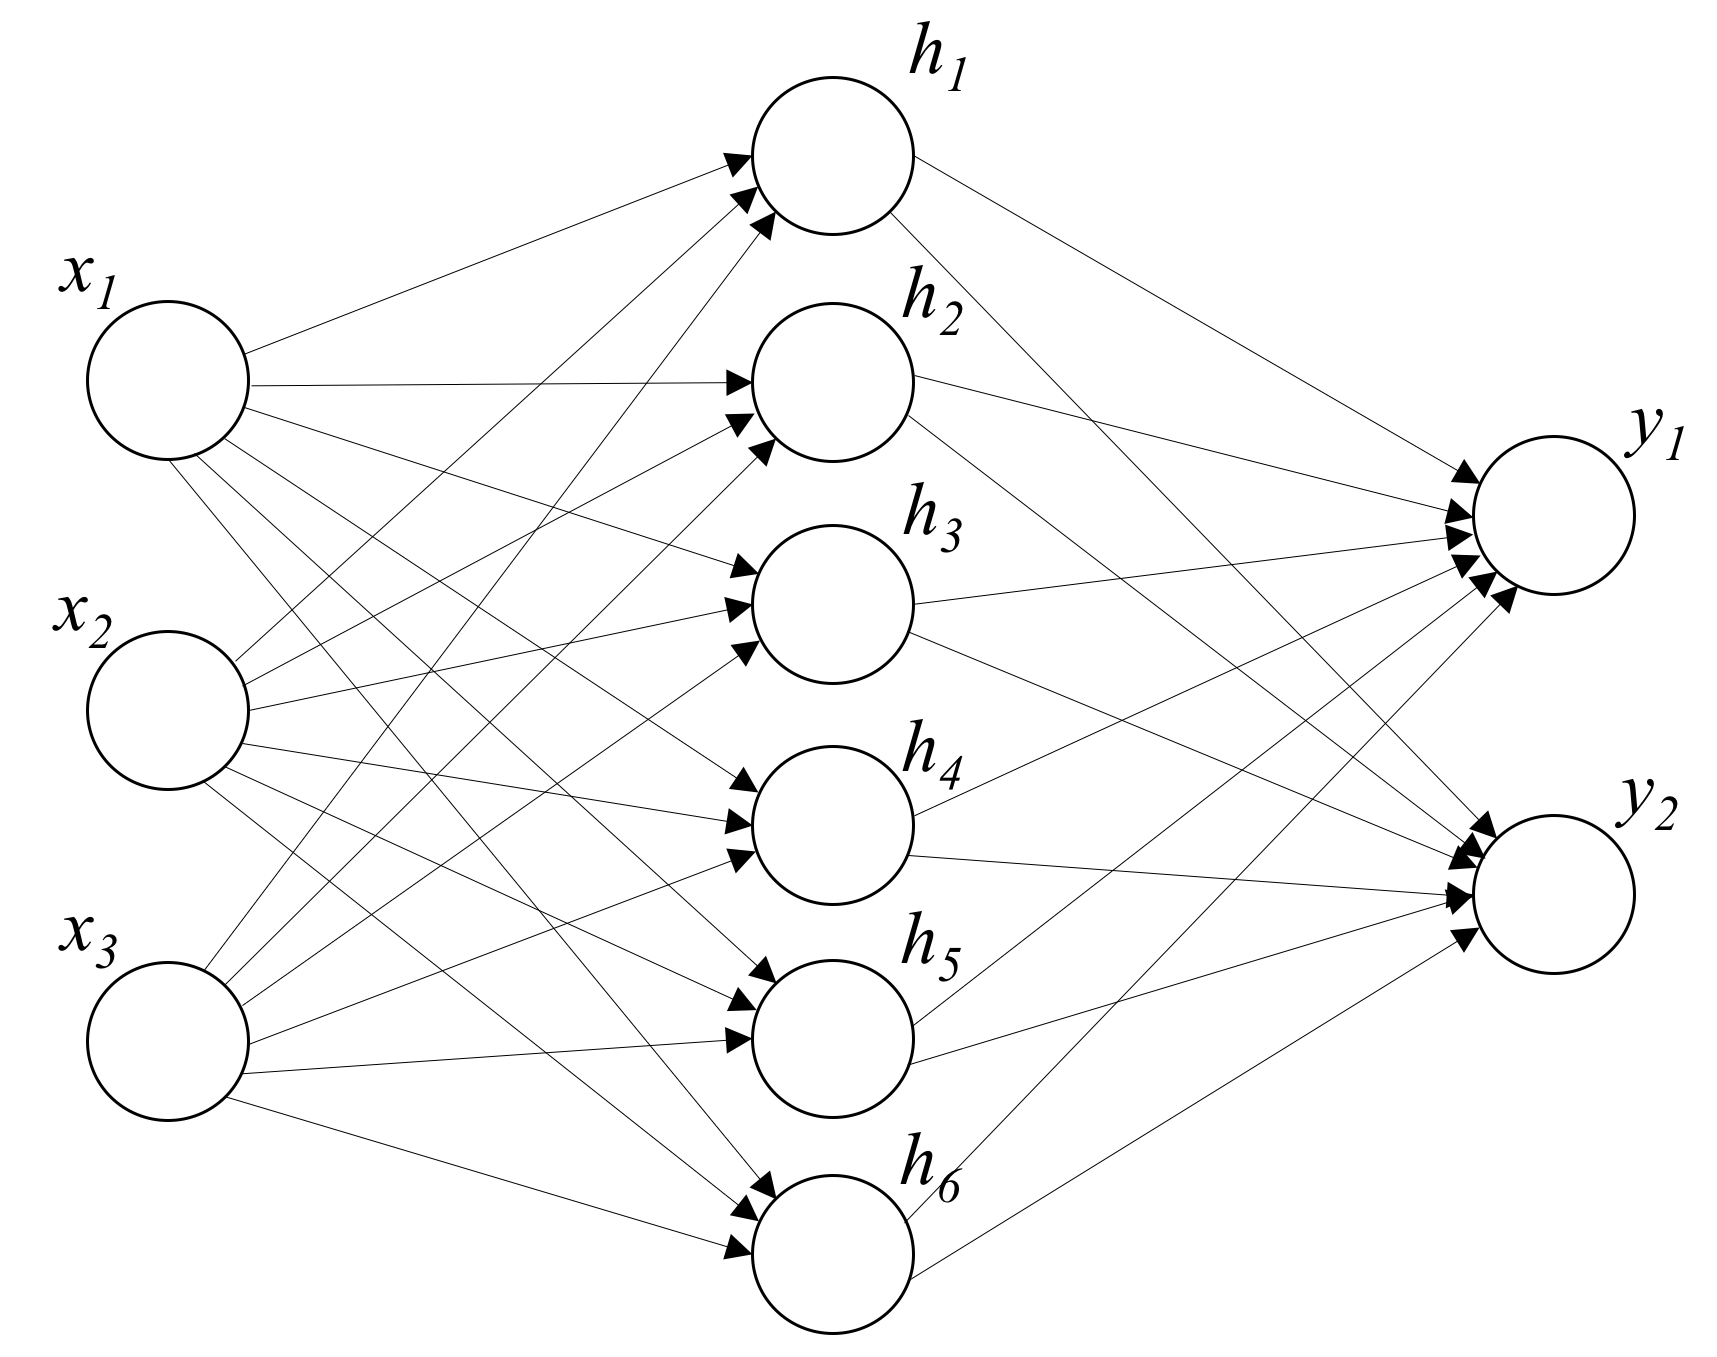
\includegraphics[scale=0.15]{/Users/pstey/Documents/latex_projects/intro_deep_learning/neural_network2.png}
	\end{center}
	\end{frame}

	\begin{frame}{Single Neuron}
	\begin{columns}
		\begin{column}{0.5\textwidth}
		A single neuron takes inputs, $x_j$, and applies the weights, $w_{\cdot j}$ to the input by computing the dot product of the vectors $x$ and $w$. The result is the input to the ``activation'' function.

		\end{column}
	
		\begin{column}{0.5\textwidth}
		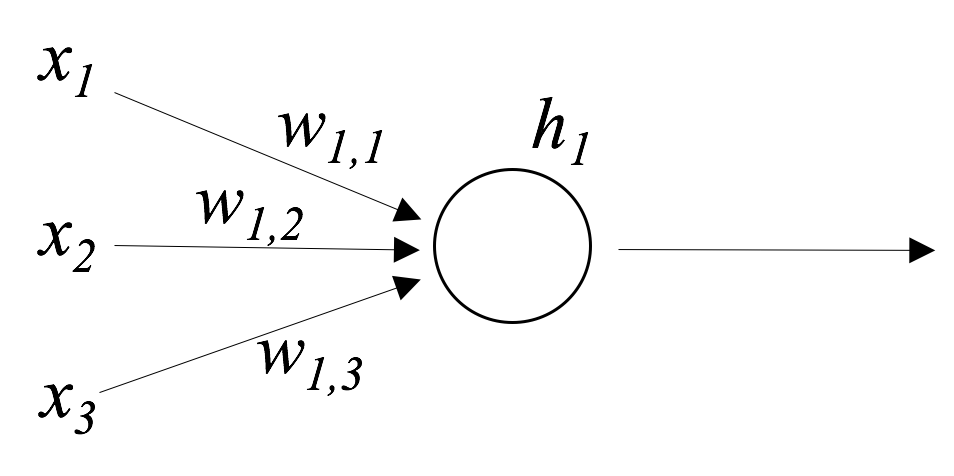
\includegraphics[scale=0.15]{/Users/pstey/Documents/latex_projects/intro_deep_learning/neuron2.png}
		\end{column}
	\end{columns}
	\end{frame}

	\begin{frame}{Activation Functions}
	
	The notion of an activation function comes again from the theoretical relationship to neurons in the brain.
	\vspace{2em}
	
	Activation functions are analogous to ``link'' functions in generalized linear models (GLMs). 
	
	\vspace{2em} 
	In fact, one common activation function is the sigmoid function, which is just our old friend the logistic function which you are using when you fit logistic regression models.
	\end{frame}
	
	
	\begin{frame}{Purpose of Activation Functions}
	
	There are a few reasons we use activation functions.	
	\vspace{2em}
	
	The most basic reason is that---like link functions in GLMs---we want to take some linear predictor and transform it so that it is bounded appropriate. For instance, the value of logistic function is in the range $(0, 1)$. 
	
	\vspace{2em}
	
	And the second key reason is that this allows us to introduce non-linearities. Recall that a neural network (like many statistical or machine learning models) is trying to approximate a data-generating mechanism. So we are trying to approximate a function that might be very complex and include many non-linearities.
	\end{frame}
	
	
	\begin{frame}{Common Activation Functions}
	Some common activation functions include the following: 
	\vspace{1em}
	\begin{enumerate}
		\item Sigmoid (i.e., logistic)
		\item Hyperbolic tangent: $tanh(\cdot)$
		\item Rectified linear unit (ReLU)
		\item Parametric Rectified linear unit (PReLU)
		\item Leaky ReLU
	\end{enumerate}
	\end{frame}




\section{Species of Neural Networks}
	\subsection{Convolutional Neural Network}

	\begin{frame}{Convolutional Neural Networks}
	\begin{center}
		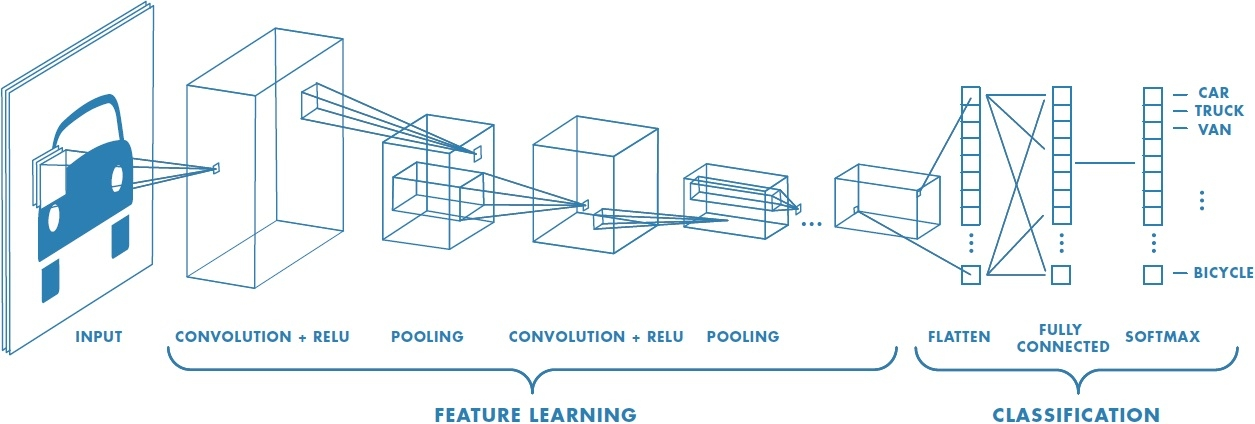
\includegraphics[scale=0.25]{/Users/pstey/Documents/latex_projects/intro_deep_learning/cnn2.jpg}
	\end{center}
	\vspace{3em}
	\Tiny{Source: https://www.mathworks.com/discovery/convolutional-neural-network.html}
	\end{frame}

	\subsection{Recurrent Neural Network}

	\begin{frame}{Recurrent Neural Networks}
	\begin{center}
		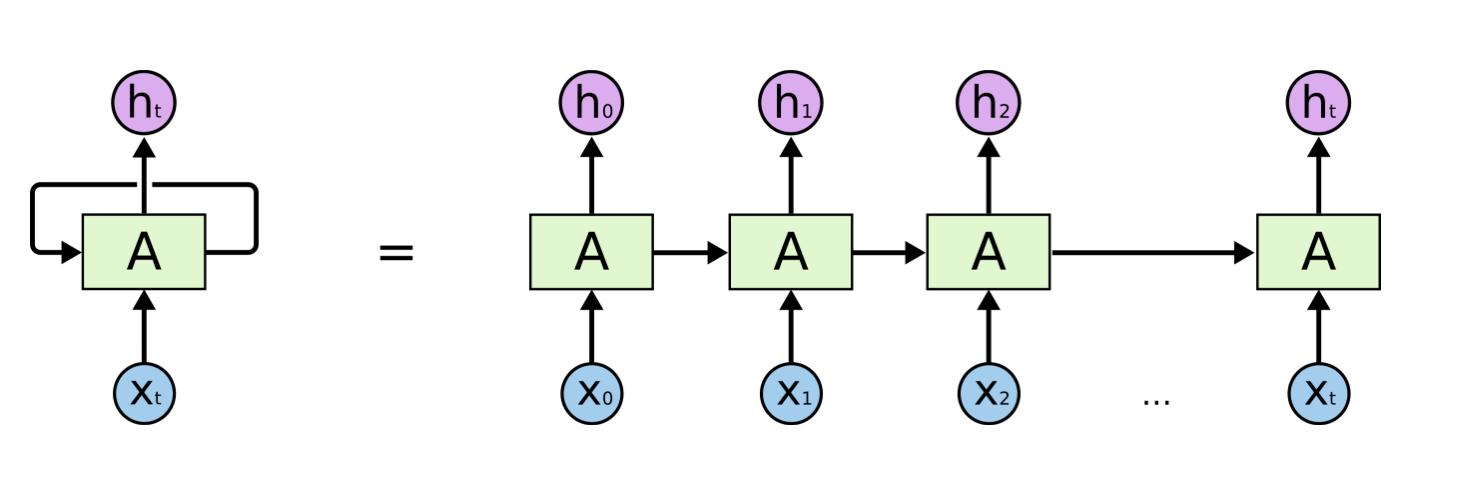
\includegraphics[scale=0.20]{/Users/pstey/Documents/latex_projects/intro_deep_learning/rnn_unrolled2.png}
	\end{center}
	\end{frame}


\subsection{Advantages of Neural Networks}

\subsection{Disadvantages of Neural Networks}

\subsection{Perceptron}


\section{Applications of Neural Networks}

\subsection{Computer Vision}
		
\subsection{Natural Language Processing}

\subsection{Speech Recognition}


\section{Summary}

\subsection{When to use Neural Networks}
	\begin{frame}{When to use neural networks}
		Conditions under which you might consider using neural networks:
		\begin{enumerate}
			\item Have a huge amount of labeled training data
			\item Image classification (with huge amount of labeled images)
			\item Certain NLP tasks
			\item Some signal processing problems
		\end{enumerate}
	\end{frame}

	\begin{frame}{When \textit{not} to use neural networks}
		Probably should \textbf{not} use neural networks when:
		\vspace{1em}
		\begin{enumerate}
			\item You have specific hypotheses you want to test
				\begin{itemize}
					\item E.g., ``\textit{Drug $X$ improves condition $Y$}''.
				\end{itemize}
			\item Interested in estimating the effect of some variable(s) on some outcome variable
			\item You have highly structured data and/or few features
		\end{enumerate}
		
		\vspace{2em}
		
		In the case of (1.) and (2.), a traditional statistical model is better. In the case of (3.), using some ensemble-of-trees method will give as-good or better results with minimal tuning.
	\end{frame}
		
\end{document}